% \documentclass{article}
\documentclass[../../outputs/main.tex]{subfiles}

% Any packages or configurations specific to this section
\usepackage{lipsum}
\usepackage{graphicx}

\begin{document}

\section{Case Study Demonstration}
% The energy price data is taken from the ComEd hourly live prices data \cite{comedLivePrices} for 10 November 2023. 

\subsection{Simulation Data: IEEE 123 Bus Test System}

We're using a Balanced Three-Phase version of the IEEE 123 Bus Test System, which has $85$ Load Nodes. Additionally, $20 \% \, (17)$ and $30 \% \, (26)$ of these load nodes also contain reactive power controllable Solar photovolatics (PVs) and Batteries respectively. Their ratings are as per \Cref{table:parameter-values}. To demonstrate the effectiveness of the proposed algorithm, the Test System has been divided into four areas on similar lines as \cite{Sadnan}. The full test system along with the area-wise division is shown in \Cref{fig:ieee123-four-area-figure}.

It is assumed that a horizon-wide forecast for loads $p^t_L$, solar power output $p^t_D$ and cost of substation power  $C^t$ is available to the distribution grid operator. \Cref{fig:inputCurve-5} shows the forecasted profiles for load, solar irradiance and cost of substation power over a $5$ time-period horizon. 

\begin{figure}[h!]
    \centering
    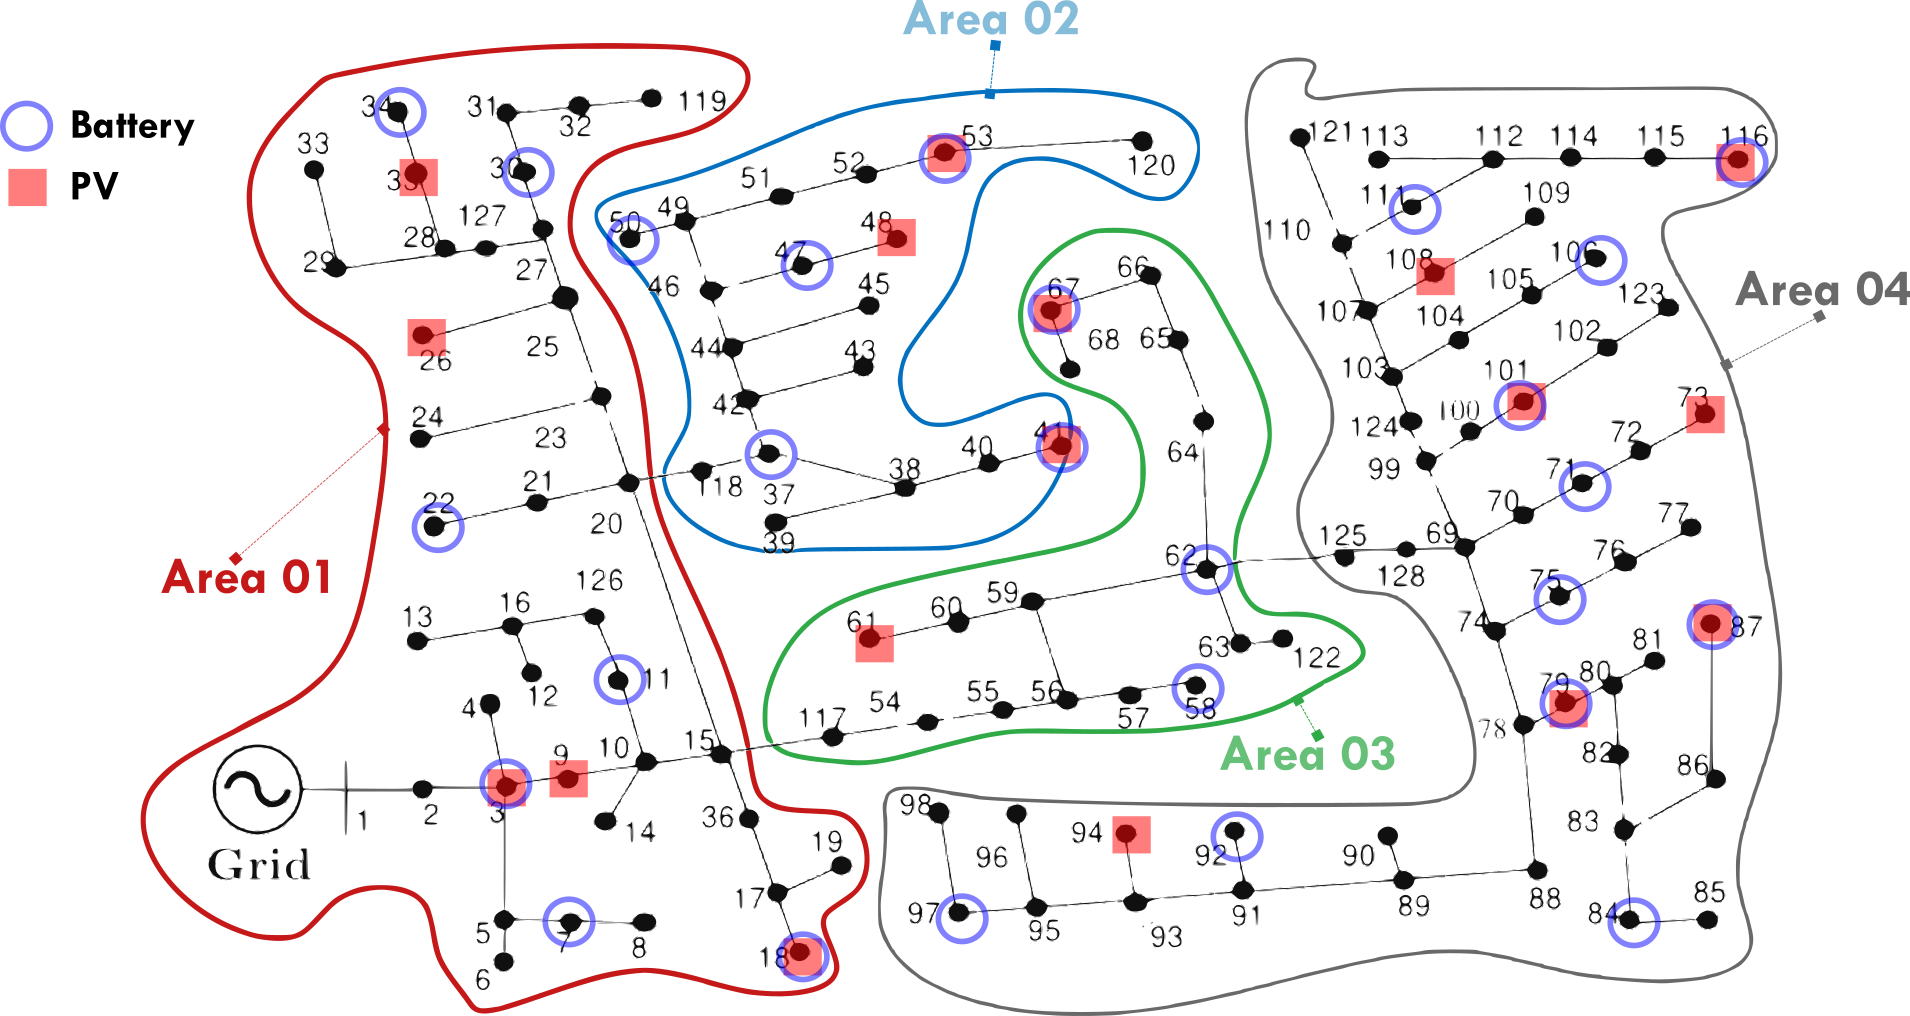
\includegraphics[width=\linewidth]{../figures/ieee123-FourAreas-pv20-batt30.png}
    \caption{IEEE 123 Node System Divided Into Four Areas}
    \label{fig:ieee123-four-area-figure}
\end{figure}

To showcase the workflow of the proposed algorithm, simulations were run for a $5$ time-period horizon. 

\begin{figure}[h!]
    \centering
    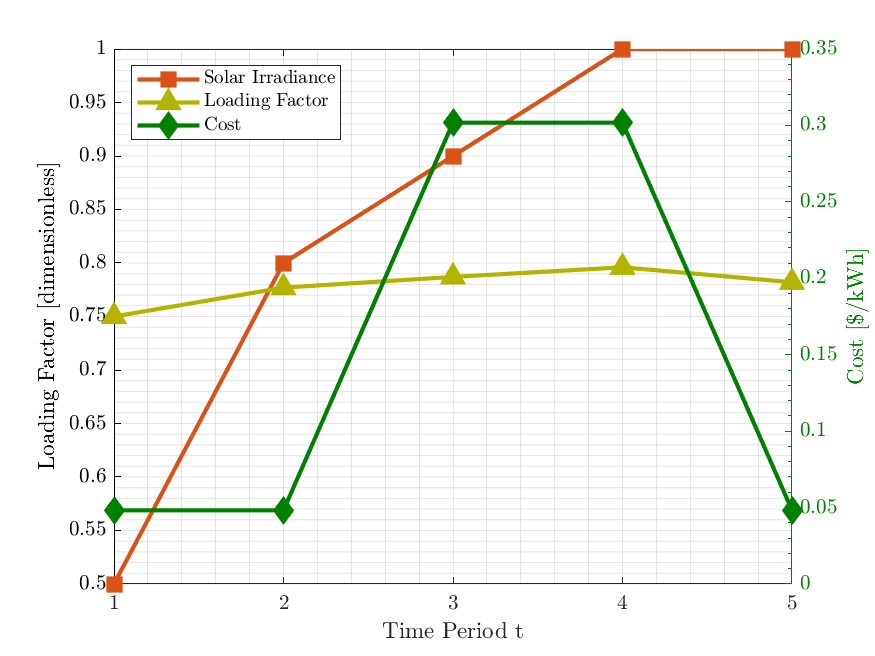
\includegraphics[height=0.25\textheight]{../figures/T5-inputCurves/InputCurves_Horizon_5.png}
    \caption{Forecasts for Demand Power, Irradiance and Cost of Substation Power over a 5 Hour Horizon}
    \label{fig:inputCurve-5}
\end{figure}

\def\ds{\rule{0pt}{1.5ex}} % this will lower the subscript by that amount, useful for $p_{D_{R_j}}$ where otherwise p and D appear to be almost at the same level.

\begin{table}[h!]
    \centering
    \caption{Parameter Values}
    \begin{tabular}{|l|c|}
    \hline
    \textbf{Parameter} & \textbf{Value} \\ \hline
    $V_{min}, V_{max}$ & 0.95, 1.05 \\ \hline
    $p_{\ds D_{R_j}}$ & $0.33 p_{\ds L_{R_j}}$ \\ \hline
    $S_{D_{R_j}}$ & $1.2 p_{\ds D_{R_j}}$ \\ \hline
    $P_{B_{R_j}}$ & $0.33 p_{\ds L_{R_j}}$ \\ \hline
    $B_{R_j}$ & $T_{fullCharge} \times P_{B_{R_j}}$ \\ \hline
    $T_{fullCharge}$ & 4 h \\ \hline
    $\Delta t$ & 1 h \\ \hline
    $\eta_C, \eta_D$ & 0.95, 0.95 \\ \hline
    $soc_{min}, soc_{max}$ & 0.30, 0.95 \\ \hline
    $\alpha$ & 0.001 \\ \hline
    \end{tabular}
    \label{table:parameter-values}
\end{table}

\subsection{Simulation Workflow}

We use MATLAB 2023a to set up our simulations. This includes both the high level algorithms as well as calling the optimization solver. We use MATLAB's \texttt{fmincon} function to parse nonlinear nonconvex optimization problem described by \crefrange{eq:genCost_withSCD}{eq:modelEndsHere-and-lim_Bj} and the SQP optimization algorithm to solve it. Once the simulations are completed and resulting optimial control variables obtained, they are passed through an OpenDSS engine (which already has the known system data and forecasted values configured) in order to check for the feasiblity of the results. The associated code may be found \href{https://github.com/Realife-Brahmin/MultiPeriod-DistOPF-Benchmark}{here}.

% \href{https://t.ly/dUCfC}{here}. % shortened link

\end{document}
